\section{Introduction}
\begin{itemize}
    \item Format of the IP header.
    \item Format of IP addresses.
    \item Different types of traffic: unicast, broadcast, and multicast.
    \item Subnet mask.
\end{itemize}


%----------------------------------------------------------------------------------------
\section{The IP header}
\begin{itemize}
    \item The network layer:
        \begin{itemize}
            \item The network layer is responsible for routing packets to their destination and for Quality of Service.
                \begin{itemize}
                    \item Quality of service: when some levels of trafic require better quality of traffic, so for example, a voice or video is sensitive to delay so it will need a better quality service than something like email.
                \end{itemize}
            \item IP (Internet Protocol) is the best known Layer 3 Protocol. IPv4 is the focus of this section.
                \begin{itemize}
                    \item There is also IPv6 which is a newer protocol.
                \end{itemize}
            \item It is a connectionless protocol with no acknowledgements at Layer 3.
                \begin{itemize}
                    \item You can have reliable traffic by using TCP at layer 4, but itself has no acknowledgement. You can also have reliable traffic by building it into the upper layers.
                \end{itemize}
            \item Other Layer 3 Protocols include ICMP (Internet Control Message Protocol) and IPSec.
                \begin{itemize}
                    \item The ICMP is used for troubleshooting, IPSec is for secure and encrypted communications. There are others as well but these are the most common.
                \end{itemize}
        \end{itemize}
    
    \item IP addressing:
        \begin{itemize}
            \item IP addressing is a logical addressing scheme which is implemented at layer 3.
            \item The network designer uses IP addressing to partition the overall network into smaller 'subnets'.
            \item This improves performance and security and makes troubleshooting easier.
                \begin{itemize}
                    \item It improves performance because instead of having a big network we have a set of small 'subnets' and we can keep the traffic to the particular subnet that it needs to be on rather than everywhere.
                    \item We also get better security. Example: if we have accounting servers, we can put it in it's own subnet and better control who has access to those servers.
                    \item Troubleshooting becomes easier because we now know that if a problem occurs it will show only on that particular subnet rather than in the entire network.
                \end{itemize}
            \item Layer 2 MAC addresses use one big flat addressing scheme. There is no logical separation between networks at layer 2, it's done at Layer 3.
                \begin{itemize}
                    \item IP addressing is a logical addressing scheme, whereas MAC addresses are a big flat scheme.
                \end{itemize}
        \end{itemize}
    
    \item OSI Reference Model - Encapsulation:
        \begin{figure}[H]
            \centering
            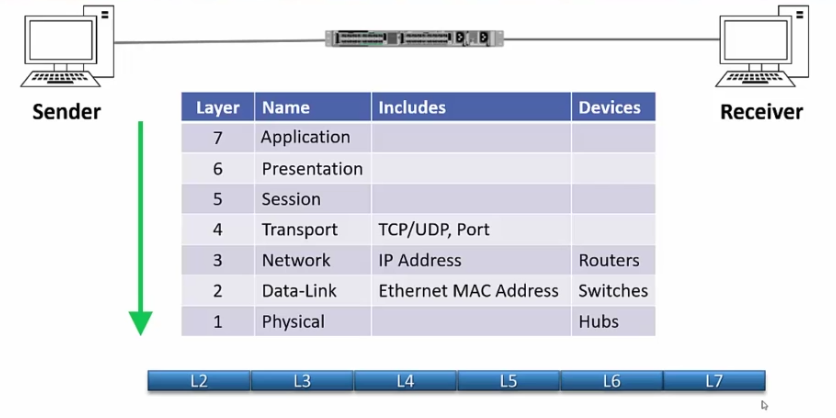
\includegraphics[width=0.4\textwidth]{./Figs/2022-01-05-22-39-03.png}
        % 	\caption{}
        \end{figure}
    
    \item The IP header:
        \begin{figure}[H]
            \centering
            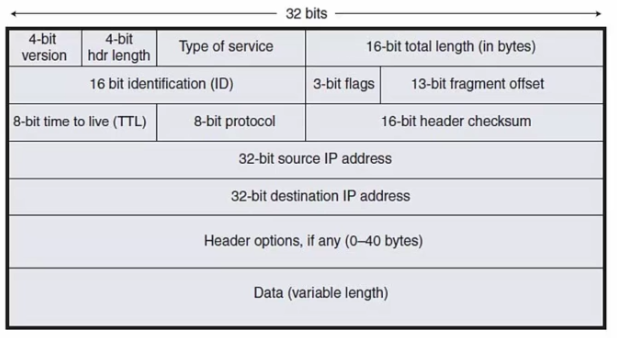
\includegraphics[width=0.4\textwidth]{./Figs/2022-01-05-22-39-43.png}
        % 	\caption{}
        \end{figure}
        \begin{itemize}
            \item Version (4 bit): Ip version 4 or version 6.
            \item header length: (4 bit): the length of the header.
            \item Type of service: this is actually the quality of servie information, we can mark the packet with quality of service information so that we can make routers respond to this information.
            \item total length (16 bit): length of the packet.
            \item The second row of information (identification, flags, fragment offset) handles the fragments. Fragments: packets have a maximum size, when the information that is to be sent exceds the maximum packet size it is split up into several packets and sends them, these split up packets are called fragments.
            \item time to live: everytime a packet goes through a router, the router will decrement the TTL by one, if it goes down to 0 the router drops the packet. This is to avoid routing loops, routing loops are when a packet is being sent through the same routers endlessly without being able to find its destination because of some error, to prevent this the time to live is decreased to be able to discard the packet once it has reached the maximum amount of times. This doesn't fix the problem in the network that caused the routing loop, but it will allow us to mitigate a potentially growing problem in our network.
            \item 8-bit protocol: specify the layer 4 information type, usually TCP or UDP.
            \item Check sum: to ensure that the packet has not been corrupted in transit.
            \item source IP address (32 bit): from where the packet is comming from.
            \item destination IP address (32 bit): to where it is headed.
            \item Header options (0-40 bytes): this field is used to send any additional information in the header, it is not typically used.
            \item Data (variable length): the actual data being transmitted.
        \end{itemize}
\end{itemize}


%----------------------------------------------------------------------------------------
\section{Unicast, Broadcast, and Multicast Traffic}
\begin{itemize}
    \item Unicast, Broadcast, and Multicast Traffic
        \begin{itemize}
            \item There are 3 main IP traffic types: unicast, broadcast, adn multicast.
            \item Unicast traffic is to a single destination host.
            \item Broadcat traffic is to all hosts on a subnet.
            \item Multicast traffic is to multiple interested hosts.
        \end{itemize}
    
    \item Unicast traffic:
        \begin{figure}[H]
            \centering
            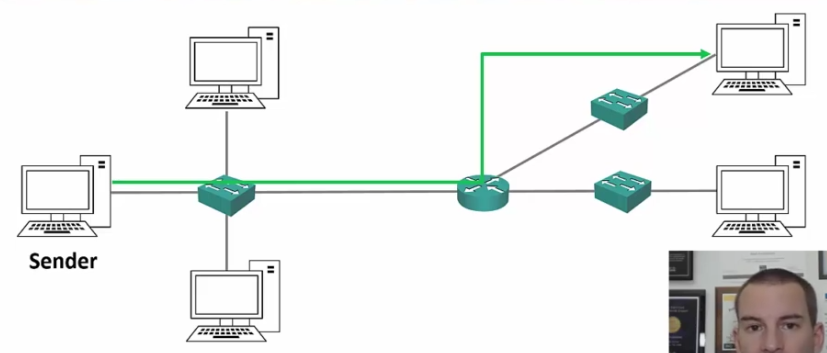
\includegraphics[width=0.4\textwidth]{./Figs/2022-01-05-23-14-20.png}
        % 	\caption{}
        \end{figure}
        \begin{itemize}
            \item The traffic is coming from a sender, and is going just to one receiver.
        \end{itemize}
    
    \item Broadcast traffic:
        \begin{figure}[H]
            \centering
            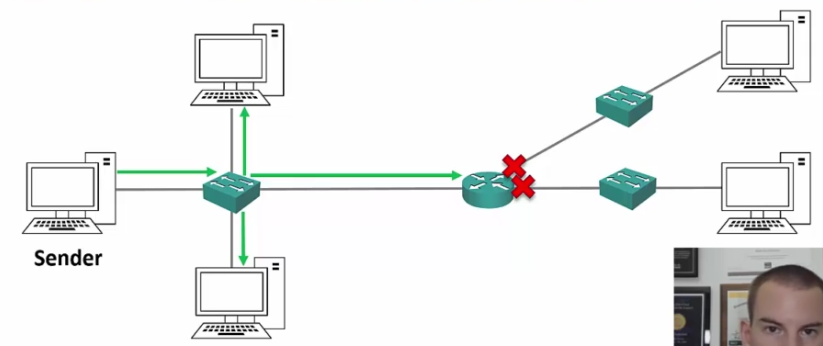
\includegraphics[width=0.4\textwidth]{./Figs/2022-01-05-23-18-22.png}
        % 	\caption{}
        \end{figure}
        \begin{itemize}
            \item The sender sends ONE copy of the traffic that will come into the switch, and then it gets to all of the hosts connected to the switch.
            \item *Important: when a broadcast is sent in a subnetwork, routers do not forward broadcast traffic, only switches do that.
        \end{itemize}
    
    \item Unicast Traffic to Multiple Hosts:
        \begin{figure}[H]
            \centering
            
        % 	\caption{}
        \end{figure}
        \begin{itemize}
            \item With unicast you send out one individual copy of the requested data to the other hosts. This can potentially become expensive because of the extra bandwidth and can cause a lot of overhead. 
                \begin{figure}[H]
                    \centering
                    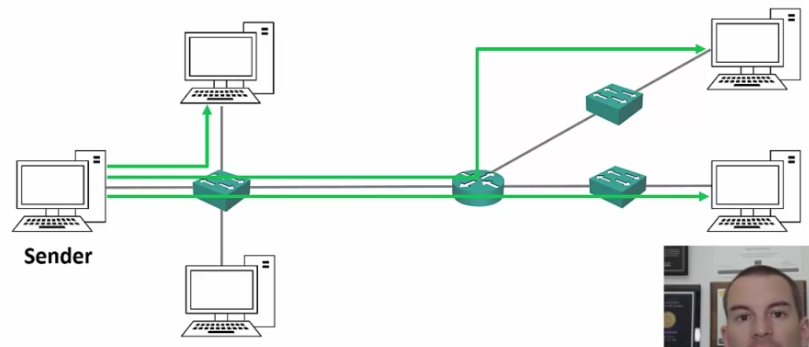
\includegraphics[width=0.4\textwidth]{./Figs/2022-01-05-23-24-16.png}
                % 	\caption{}
                \end{figure}
            \item When you unicast a message to several computers you send to each individual destination host a different copy. With multicast you send one copy that goes to several different receivers, with this arrangement you don't produce a different copy for all of the interested receivers, you send out one, and that one copy gets forwarded to all the different receivers.
                \begin{figure}[H]
                    \centering
                    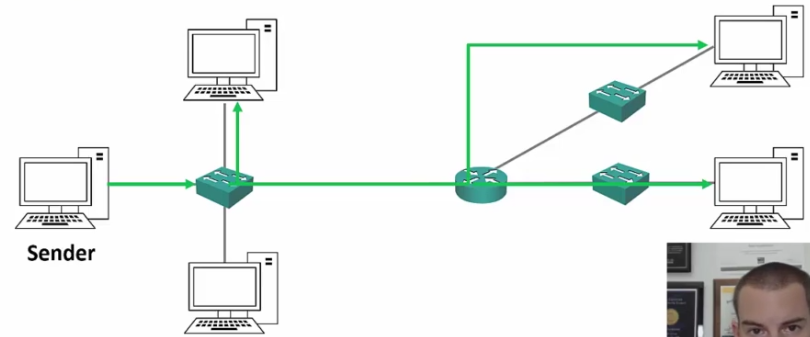
\includegraphics[width=0.4\textwidth]{./Figs/2022-01-05-23-25-35.png}
                % 	\caption{}
                \end{figure}
            
            \item Multicast goes to multiple receivers but only if the receivers request it, with broadcast all hosts on a network get the data regardless of request, multicast is targeted. 
            \item *Analogy: multicast is like tunning to a radio station, you have to tune in to get that particular radio station.
        \end{itemize}
\end{itemize}


%----------------------------------------------------------------------------------------
\section{Converting from decimal to binary}
\begin{itemize}
    \item Counting in decimal:
        \begin{itemize}
            \item Humans are conditioned to count in decimal.
            \item For each 'column' in a number we have 10 possible choices, from 0-9.
            \item Every time we add a column to the left, the value is multiplied by 10.
            \item We start with '1s' as the further right column.
                \begin{figure}[H]
                    \centering
                    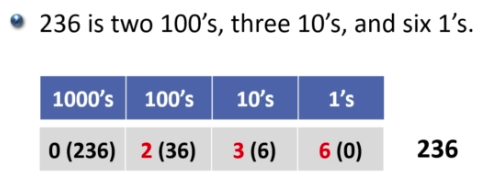
\includegraphics[width=0.4\textwidth]{./Figs/2022-01-05-23-39-44.png}
                % 	\caption{}
                \end{figure}
            
            \item Writing 236 implies the following: 
        \end{itemize}
    
    \item Counting in binary:
        \begin{itemize}
            \item Computers work in binary.
            \item Electrical impulses are either off or on, so there's only two choices (0 or 1), unlike 10 in decimal (0-9).
            \item For each 'column' in a number we have 2 possible choices, 0 or 1.
            \item Everytime we add a column to the left, the value is multiplied by 2.
            \item In this case the columns are like so:
                \begin{figure}[H]
                    \centering
                    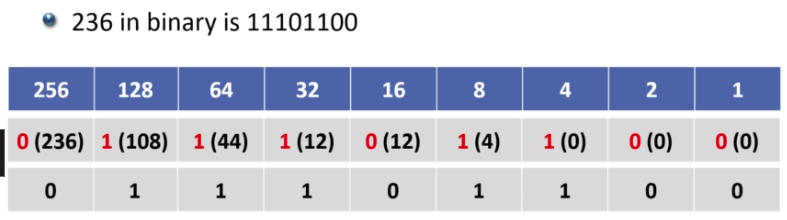
\includegraphics[width=0.4\textwidth]{./Figs/2022-01-05-23-41-13.png}
                % 	\caption{}
                \end{figure}
            
            \item The number we are going to get in the end is 11101100. We do this like so. A final check is that at the end of the process you should have 0 left over.
        \end{itemize}
\end{itemize}


%----------------------------------------------------------------------------------------
\section{IPv4 Addresses}
\begin{itemize}
    \item IPv4 Addresses:
        \begin{itemize}
            \item An IPv4 address is 32 bits long.
            \item It is written as 4 'octets' in dotted decimal format.
            \item For example 192.168.10.15
            \item Each octet is 8 bits long, 4 octets are 32 bits.
        \end{itemize}
    
    \item Seeing your IP address:
        \begin{figure}[H]
            \centering
            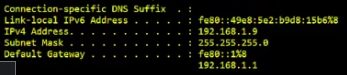
\includegraphics[width=0.4\textwidth]{./Figs/2022-01-05-23-49-32.png}
        % 	\caption{}
        \end{figure}
        \begin{itemize}
            \item If we were to type 'ipconfig' in cmd (windows) or 'ifconfig' in the terminal (linux and macos) we would get all sorts of information regarding the IP address.
            \item IPv4 address is printed, the subnetmask is also printed, and the default gateway is printed. A default gateway is used when traffic is going to another host on another subnet, when the destination host is in the same subnet it can get there directly but if it is not it will go through a router and enter a different subnet, the default gateway in that case is the router to the other subnets and networks. 
            \item To see the default gateway on linux or macos enter 'ip route'.
            \item To get your ip in Cisco OS, enter the enable prompt and type 'show ip interface brief'.
        \end{itemize}
    
    \item Static and automatic addressing:
        \begin{itemize}
            \item The IP address is usually se manually on servers, printers and network devices such as routers and switches. On desktop computers it is usually assigned automatically through the Dynamic Host Configuration Protocol (DHCP).
                \begin{itemize}
                    \item The reason you want to get your IP is set automatically on desktops is because you would not want to set it up manually because you would need to see which IP address is not in use and then set it up, instead you are automatically assigned one. With servers and routers you can do it manually because you they are fewer and they are going to almost always be the same IP address.
                \end{itemize}
            \item To understand how the logical separation between subnets works, you need to understand the IP address in binary.
                \begin{itemize}
                    \item 
                \end{itemize}
        \end{itemize}
\end{itemize}
